\documentclass[11pt,compress,t,notes=noshow, xcolor=table]{beamer}
\input{../../style/preamble}
\input{../../latex-math/basic-math}
\input{../../latex-math/basic-ml}

\newcommand{\sens}{\mathbf{A}} % vector x (bold)

\newcommand{\batilde}{\tilde{\mathbf{a}}}
\newcommand{\Px}{\mathbb{P}_{x}} % P_x
\newcommand{\Pxj}{\mathbb{P}_{x_j}} % P_{x_j}
\newcommand{\indep}{\perp \!\!\! \perp} % independence symbol
% ml - ROC
\newcommand{\np}{n_{+}} % no. of positive instances
\newcommand{\nn}{n_{-}} % no. of negative instances
\newcommand{\rn}{\pi_{-}} % proportion negative instances
\newcommand{\rp}{\pi_{+}} % proportion negative instances
% true/false pos/neg:
\newcommand{\tp}{\# \text{TP}} % true pos
\newcommand{\fap}{\# \text{FP}} % false pos (fp taken for partial derivs)
\newcommand{\tn}{\# \text{TN}} % true neg
\newcommand{\fan}{\# \text{FN}} % false neg

\newcommand{\Tspace}{\mathcal{T}}
\newcommand{\tv}{\mathbf{t}}
\newcommand{\tj}{\mathbf{t}_j}

\usepackage{multicol}
\usepackage{color,colortbl} 
\definecolor{putblue}{RGB}{0,0,124}
\definecolor{putred}{RGB}{204,33,69}

\usetikzlibrary{mindmap,trees}
\usetikzlibrary{decorations.pathreplacing}
\usetikzlibrary{decorations.pathmorphing}
\usetikzlibrary{arrows}
\usetikzlibrary{positioning}
\usetikzlibrary{decorations.text}
\usetikzlibrary{decorations.markings}
\usetikzlibrary{decorations.shapes}
\usetikzlibrary{shapes,snakes}
\usetikzlibrary{calc,trees,positioning,arrows,chains,shapes.geometric,
	decorations.pathreplacing,decorations.pathmorphing,shapes,matrix,shapes.symbols}
\usetikzlibrary{shapes.misc}


\newcommand{\titlefigure}{figure/mean_relation}
\newcommand{\learninggoals}{
  \item Know how to leveraging and constucting the target similarity in multi-target learning
%  \item 
}

\title{Advanced Machine Learning}
\date{}

\begin{document}

\lecturechapter{Methods for Multi-Target Prediction: Part 2}
\lecture{Advanced Machine Learning}



\sloppy

\section{Similarity-exploiting methods}


\begin{frame}{Kronecker kernel ridge regression}
	\footnotesize
	\begin{itemize}
%		
	\item In the case of multi-target prediction with target features one typically uses kernel methods for learning.
%		
	\item In particular, one considers the following pairwise model representation in the primal: 
		\begin{equation*}
			\label{eq:pairwise}
			f(\xv,\tv) = \bm\omega^\top \left(\phi(\xv) \otimes \psi(\tv) \right) ,
		\end{equation*}
%	
	where $\phi$ is some feature map for the features and $\psi$ is a feature map for the target (features) and $\otimes$ is the Kronecker product. \textbf{TODO: Define $\tv$}
%
	\item This leads to the Kronecker product pairwise kernel in the dual:
%	
	\begin{eqnarray*} 
		f(\xv,\tv)= \sum_{(\xv',\tv') \in \D} \alpha_{(\xv',\tv')}  \cdot  k(\xv,\xv') \cdot g(\tv,\tv')  = \sum_{(\xv',\tv') \in \D} \alpha_{(\xv',\tv')} \Gamma((\xv,\tv),(\xv',\tv')),
	\end{eqnarray*}
%
	where $k$ is the kernel for the feature map $\phi,$  $g$ the kernel for the feature map $\psi$  and $\alpha_{(\xv',\tv')}$ are the dual parameters, which can be found by least-squares minimization:
%	 
	$$ \min_{\bm{\alpha}} \, ||\bm{\Gamma}\bm{\alpha} -\bm{z} ||^2_2 +\lambda\bm{\alpha }^\top \bm{\Gamma}\bm{\alpha}, $$
%	
	where $\bm{z} = \mathrm{vec}{(Y)}.$
%
%	\item Idea: Model the joint kernel as a product of an instance kernel $k(\cdot,\cdot)$ and a target kernel $g(\cdot,\cdot)$: 
%		$$\Gamma((\xv,\tv),(\xv',\tv')) = k(\xv,\xv') \cdot g(\tv,\tv')$$
%
	\item This approach is commonly used in the zero-shot learning framework.

%
\end{itemize}
%	
	{\tiny Stock et al., A comparative study of pairwise learning methods based on kernel ridge regression, Neural Computation 2018.}
%	
\end{frame}



\begin{frame}{Exploiting relations in regularization terms}
	\footnotesize
%
	\begin{center}
		\includegraphics[width=\textwidth]{figure/targetrelations}
	\end{center} 
%	
	\begin{itemize}
%		
		\item 	Graph-based regularization is an approach that can be applied to the tree types of relations in the targets: 
		%
		\begin{equation*}
			\min_\Theta \|Y - \Phi \Theta \|^2_F + \lambda \sum_{m=1}^l \sum_{m' \in \mathcal{N}(m)} \|\thetab_m - \ \thetab_{m'}\|^2,
		\end{equation*}
		%
		where $\mathcal{N}(j)$ is the set of targets that are related to target $j.$
        \item Recall that the graph or tree is given as prior information.
%		
		\item Can also be used in a weighted version taking the similarities (or correlations) into account.
%		
	\end{itemize}
	
%
	{\tiny Gopal and Yang, Recursive regularization for large-scale classification with hierarchical and graphical dependencies, KDD 2013.}
\end{frame}

\begin{frame}{Hierarchical multi-label classification}
	\small
	\vspace{-0.2cm}
	\begin{center}
		\includegraphics[width=\textwidth]{figure/hloss}
	\end{center}
	
	\vspace{-0.2cm}
	\begin{minipage}{0.75\textwidth}   
	\begin{itemize}
%		
		\item %	
		Hierarchies can also be used to define specific loss functions, such as the Hierarchy-loss: 
		%	
		$$L_{Hier}(\yv, f) = \sum_{m: y_m \neq \hat{y}_m} c_m \, \mathds{1}_{ [\textit{anc}(y_m) = \textit{anc}(\hat{y}_m)]  },$$
		%	
		where $c_m$ are costs depending on the depth of node $m$, and $\hat{y}_m$ are the predicted labels.
		%	
%		
	\end{itemize}
\end{minipage}
\begin{minipage}{0.2\textwidth}    
	\begin{center}
		%    	
		\includegraphics[width=0.99\textwidth,trim = 0 0 100 20,clip]{figure/Slide5}
		%    	
	\end{center}
\end{minipage}
\begin{itemize}
%	
	\item This is rather common in multi-label classification problems.
%	
\end{itemize}

	{\tiny Bi and Kwok, Bayes-optimal hierarchical multi-label classification, IEEE Transactions on Knowledge and Data Engineering, 2014.}
%
\end{frame}



\section{Similarity-constructing methods}




\begin{frame}
	\frametitle{Probabilistic classifier chains}
	
	\begin{itemize}
		\item Estimate the \alert{joint} conditional distribution $\P(\yv ~|~  \xv)$. 
		\item For optimizing the \alert{subset 0/1} loss:  $$ L_{0/1}(\yv, \hat{\yv}) = \mathds{1}_{[\yv \ne \hat{\yv}]}$$
		\item Repeatedly apply the \emph{product rule} of probability:
		$$
		\P(\yv ~|~ \xv) = \prod_{j=m}^{l} \P(y_m ~|~ \xv, y_1, \ldots,y_{m-1}) \, .
		$$
		\item  Learning relies on constructing \alert{probabilistic classifiers} for estimating 
		$$
		\P( y_m|\xv, y_1, \ldots,y_{m-1}) \,,
		$$
		{independently} for each $m = 1, \ldots, l$. 
		%\item One can use scoring functions $f_i(\xv^\prime,y_i)$ and use logistic transformation.
		%\item By using the linear models, the overall scoring function takes the form:
		%$$
		%f(\xv,\yv) = \sum_{i=1}^m f_i(\xv, y_i) + \sum_{y_k,y_l} \! f_{k,l}(y_k,y_l) 
		%$$
	\end{itemize}
\end{frame}

\begin{frame}[fragile]
	\frametitle{Probabilistic classifier chains}
	\begin{itemize}
		\item Inference relies on exploiting a probability tree:
	\end{itemize}
	\vspace{0.1cm}
	\begin{center}
		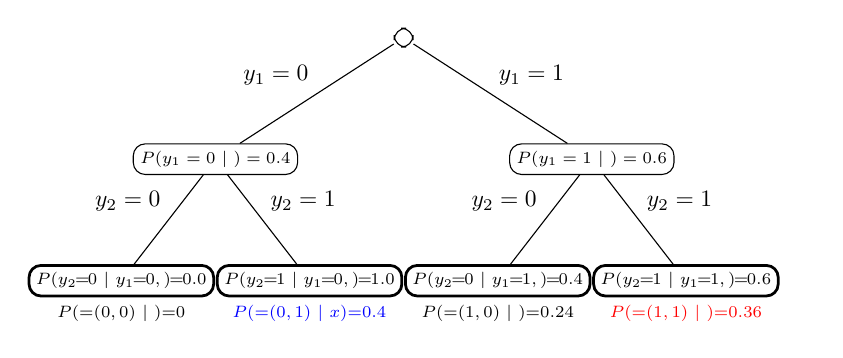
\begin{tikzpicture}[scale = 0.85,every node/.style={scale=0.85},
			regnode/.style={circle,draw,minimum width=1.5ex,inner sep=0pt},
			leaf/.style={circle,fill=black,draw,minimum width=1.5ex,inner sep=0pt},
			pleaf/.style={rectangle,rounded corners=1ex,draw,font=\scriptsize,inner sep=3pt,line width=1pt},
			pnode/.style={rectangle,rounded corners=1ex,draw,font=\scriptsize,inner sep=3pt},
			rootnode/.style={rectangle,rounded corners=1ex,draw,font=\small,inner sep=4pt},
			level/.style={sibling distance=16em/#1, level distance=12ex}
			]
			\node (z) [rootnode] {$\xv$}
			child {node (a) [pnode] {$P(y_1=0 ~|~ \xv)=0.4$} 
				child {node [label=below:{\scriptsize \thickmuskip=0mu $P(\yv=(0,0)~|~ \xv)=0$}] (b) [pleaf] {\thickmuskip=-1.5mu $P(y_2=0 ~|~ y_1=0, \xv)=0.0$} edge from parent node[above left]{$y_2=0$}}
				child {node [label=below:{\color{blue} \scriptsize \thickmuskip=0mu $P(\yv=(0,1) ~|~ x)=0.4$}] (g) [pleaf] {\thickmuskip=-1.5mu $P(y_2=1 ~|~ y_1=0, \xv)=1.0$} edge from parent node[above right]{$y_2=1$}}
				edge from parent node[above left]{$y_1=0$}
			}
			child {node (j) [pnode] {$P(y_1=1 ~|~ \xv)=0.6$}
				child {node [label=below:{\scriptsize \thickmuskip=0mu $P(\yv=(1,0) ~|~ \xv)=0.24$}] (k) [pleaf] {\thickmuskip=-1.5mu $P(y_2=0 ~|~ y_1=1, \xv)=0.4$} edge from parent node[above left]{$y_2=0$}}
				child {node [label=below:{\color{red} \scriptsize \thickmuskip=0mu $P(\yv=(1,1) ~|~ \xv)=0.36$}] (l) [pleaf] {\thickmuskip=-1.5mu $P(y_2=1 ~|~ y_1=1, \xv)=0.6$}
					{
						child [grow=right] {node (s) {} edge from parent[draw=none]
							child [grow=up] {node (t) {} edge from parent[draw=none]
								child [grow=up] {node (u) {} edge from parent[draw=none]}
							}
						}
					}
					edge from parent node[above right]{$y_2=1$}
				}
				edge from parent node[above right]{$y_1=1$}
			};
			
			%\path (s) -- (t) node [midway] {$\lambda_{2}$};
			%\path (t) -- (u) node [midway] {$\lambda_{1}$};
		\end{tikzpicture}
	\end{center}
	
	\vspace{0.1cm}
	\begin{itemize}\small
		\item For subset 0/1 loss one needs to find $
		\fbayes(\xv) = \argmax_{\yv} \P(\yv ~|~ \xv)
		$.
		\item Greedy and approximate search techniques with guarantees exist.
%		\footnote{Kumar et al., Beam search algorithms for multilabel
%	learning, Machine Learning 2013}
		\item Other losses: compute the prediction on a sample from $\P(\yv ~|~  \xv).$
%		\footnote}
		%\item[]
	\end{itemize}
{\tiny Dembczynski et al., An analysis of chaining in multi-label classification, ECAI 2012.}
	
\end{frame}



\begin{frame}{Low-rank approximation}
	
	\begin{center}
		\includegraphics[width=9cm]{figure/lowrank}
	\end{center}

	\begin{itemize}
%		
		\item Low rank materializes the idea that some structure is shared across different targets.
%
		\item 	Typically perform a low-rank approximation of the parameter matrix:
		$$\min_\Theta \|Y - \Phi \Theta \|^2_F + \lambda \, \mathrm{rank}(\Theta)$$
%		
	\end{itemize}
	{\tiny Chen et al., A convex formulation for learning shared structures from
	multiple tasks, ICML 2009.}
\end{frame}



%%%%%%%%%%%%%%%%%%%%%%%%%%%%%%%%%%%%%%%%%%%%%%%%%%%%%%%%%%%%%%%%%%%%%%%%%%%%%% 
%%%%%%%%%%%%%%%%%%%%%%%%%%%%%%%%%%%%%%%%%%%%%%%%%%%%%%%%%%%%%%%%%%%%%%%%%%%%%%  

%%%%%%%%%%%%%%%%%%%%%%%%%%%%%%%%%%%%%%%%%%%%%%%%%%%%%%%%%%%%%%%%%%%%%%%%%%%%%% 
%%%%%%%%%%%%%%%%%%%%%%%%%%%%%%%%%%%%%%%%%%%%%%%%%%%%%%%%%%%%%%%%%%%%%%%%%%%%%% 
\frame{
	\frametitle{Low-rank approximation}
	
	
	
	\begin{itemize}
		\item $\Theta$: parameter matrix of dimensionality $p \times l$ 
		\item $p$: the number of (projected) features
		\item $l$: the number of targets
		\item Assume a low-rank structure of $A$:\\
%		
		$ \qquad  \qquad\qquad \quad  U  \quad \times \qquad  V \qquad \quad  =  \qquad  A$
		\begin{center}
%					
			\includegraphics[width=0.6\textwidth,trim = 0 0 0 0,clip]{figure/uv_decomp}
%
		\end{center}
		
		\item We can write $\Theta=UV$ and $\Theta \xv = UV \xv$
		\item $V$ is a $p \times \hat{l}$ matrix
		\item  $U$ is an $\hat{l} \times l$ matrix
		
		\item $\hat{l}$ is the rank of $\Theta$
		
	\end{itemize}
	
}

\begin{frame}{Low-rank approximation: Overview of methods}
	
	\begin{itemize}
		\item Popular for multi-output regression, multi-task learning and multi-label classification.
		\item Linear as well as nonlinear methods.
		\item Algorithms: 
		\begin{itemize}
			\item Principal component analysis, Canonical correlation analysis, Partial least squares.
			\item Singular value decomposition, Alternating structure optimization.
			\item Compressed sensing, Output codes, Landmark labels, Bloom filters, Auto-encoders.
		\end{itemize}
	\end{itemize}
%   \footnote{Weston et al., Kernel dependency estimation, NIPS 2002}
% 	\footnote{Multi-label prediction via sparse infinite CCA, NIPS 2009}
%\footnote{Tai and Lin, Multilabel classification with principal label space transformation, Neural Computation 2012}
%  	\footnote{Zhou et al., Clustered Multi-Task Learning Via Alternating Structure Optimization, NIPS 2011}
%	\footnote{Hsu et al., Multi-label prediction via compressed sensing. NIPS 2009}
%	\footnote{Zhang and Schneider, Multi-label Output Codes using Canonical Correlation Analysis, UAI 2011}
%	\footnote{Balasubramanian and Lebanon, The landmark selection method for multiple output
%	prediction, ICML 2012}
%	\footnote{Ciss\'e et al., Robust bloom filters for large multilabel
%	classification tasks, NIPS 2013}
% 	\footnote{Wicker et al., A nonlinear label compression and transformation
%	method for multi-label classification using autoencoders, PAKDD 2016}
	\vspace{0.3cm}
\end{frame}


%
\endlecture
\end{document}
